\chapter{极化SAR相关理论概述}
\section{引言}
极化SAR技术通过发送和接收不同极化方式的电磁波,提供丰富的目标极化散射信息,具有全天时、全天候成像特点。因此,近年来,极化SAR在城市规划、军事探测、灾害检测、农作物监控等多个领域有着广泛的应用\citing{pramudya2019estimation,dumitru2018sar,liu2019small}。极化SAR数据具有丰富的极化特征描述方式,如何有效、全面地利用这些极化特征,增强目标散射特性的表征能力,是极化SAR图像分类任务中的关键任务\citing{dong2020attention,yang2019cnn,yang2021reconstruction}。本章将系统阐述极化SAR基本理论,内容涵盖极化电磁波数学表述方式、多种描述极化散射特征的理论与方法、目标分解理论原理及其代表性分解方法的具体实施步骤和计算流程。

% 本章将介绍极化SAR相关基础理论,包括极化电磁波的数学表征方式、极化数据散射特性的不同描述方式以及极化目标分解理论原理和集中具有代表性的目标分解方法具体计算过程。

% 同时,深度学习技术以其在遥感数据处理中的卓越表现,为极化SAR目标分类任务提供了新的思路和解决方法\citing{liu2016pol, liu2019task, bi2018graph}。本章将介绍极化SAR与深度学习方法的相关理论基础,主要包括目标散射机理介绍,极化数据的表征形式和几种典型的目标分解方法。

\section{极化电磁波表示方式}
电场与磁场的相互作用产生电磁波。在电磁波传播过程中,电场与磁场振荡平面始终保持垂直,并且都与电磁波的传播方向相垂直,如图\ref{电磁波传输过程示意图}所示:

\begin{figure}[h]
    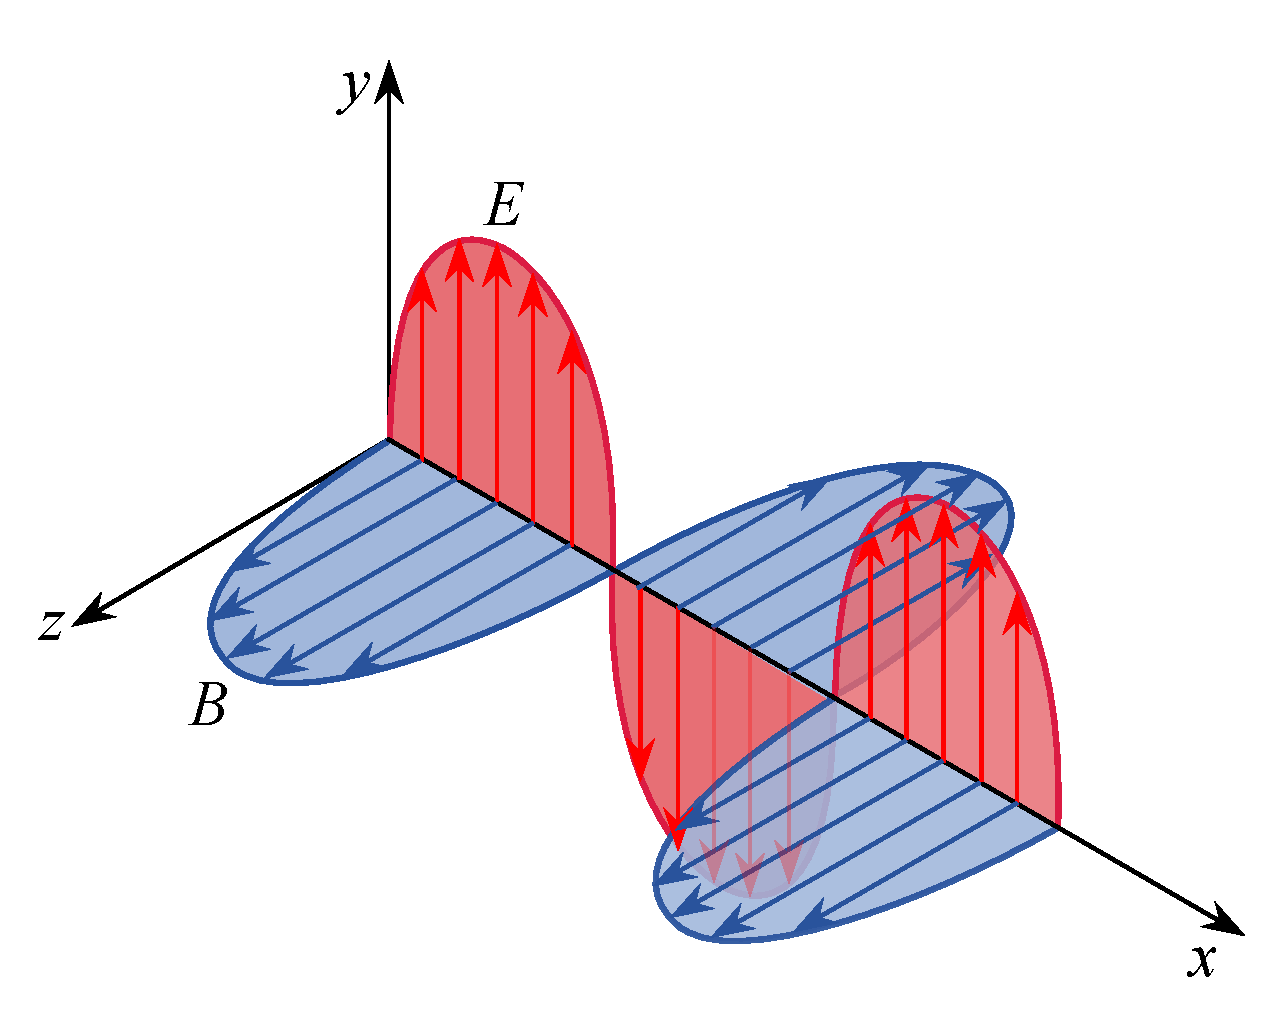
\includegraphics[width=10.3cm]{pic/chapter2/电磁波传输过程.pdf}
    \caption{电磁波传输过程示意图\citing{电磁波传播与接收}}
    \label{电磁波传输过程示意图}
\end{figure}

极化是电磁波的基本特性之一,是指在固定的空间点处,电场振荡方向随着时间的变化方式。在笛卡尔坐标系中,设定电磁波的传播方向为$\hat{z}$轴正方向,电场与磁场的关系可以使用麦克斯韦方程组表示\citing{皮亦鸣2007合成孔径雷达成像原理, 路宏敏2006电磁场与电磁波基础}:

\begin{equation}
    \label{eq:Maxwell}
    \begin{cases}
        \nabla \times \boldsymbol{H}(z,t)=\epsilon \frac{\partial \boldsymbol{E}(z,t)}{\partial t} \\
        \nabla \times \boldsymbol{E}(z,t)=-\mu \frac{\partial \boldsymbol{H}(z,t)}{\partial t}     \\
        \nabla \cdot \boldsymbol{H}(z,t)=0                                                         \\
        \nabla \cdot \boldsymbol{E}(z,t)=0                                                         \\
    \end{cases}
\end{equation}

对方程组\eqref{eq:Maxwell}第二个等式两边取旋度,有:
\begin{equation}
    \nabla \times(\nabla \times \boldsymbol{E})=-\mu \frac{\partial}{\partial t}(\nabla \times \boldsymbol{H})
\end{equation}

通过矢量恒等式$\nabla \times(\nabla \times \boldsymbol{E})=\nabla(\nabla \cdot \boldsymbol{E})-\nabla^2 \boldsymbol{E}$和方程组\eqref{eq:Maxwell}第四个等式可以得出电磁波的波动方程:
\begin{equation}
    \nabla^2 \boldsymbol{E}(z, t)-\mu \epsilon \frac{\partial^2 \boldsymbol{E}(z, t)}{\partial t^2}=0
\end{equation}

极化SAR系统与地面目标之间的距离满足远场条件,可以将极化SAR工作过程中收发的电磁波近似为平面波。通过波动方程,可以得到平面波的表达式:
\begin{equation}
    \label{平面波}
    \boldsymbol{E}(z, t)=\left[\begin{array}{c}
            E_x(z, t) \\
            E_y(z, t) \\
            0
        \end{array}\right]=\left[\begin{array}{c}
            E_{0 x} \cos \left(\omega t-k z+\delta_x\right) \\
            E_{0 y} \cos \left(\omega t-k z+\delta_y\right) \\
            0
        \end{array}\right]
\end{equation}
其中,$E_{0x}$, $E_{0y}$, $\delta_x$ 和 $\delta_y$分别表示电场在$x$与$y$方向上的幅度和初始相位,$k$ 表示传播常量。

\subsection{极化椭圆}
在空间中某个固定的点处电场矢量端点的轨迹可以用来描述电磁波的极化状态。对于某个时刻$t$,由公式\eqref{平面波}可得:
\begin{equation}
    \label{轨迹方程}
    \left(\frac{E_x(z, t)}{E_{x_0}}\right)^2-2\left(\frac{E_x(z, t) E_y(z, t)}{E_{x_0} E_{y_0}}\right) \cos (\delta)+\left(\frac{E_y(z, t)}{E_{y_0}}\right)^2=\sin ^2(\delta)
\end{equation}
其中,$\delta=\delta_x-\delta_y$,$-\pi \leqslant \delta \leqslant \pi$。

\begin{figure}[h]
    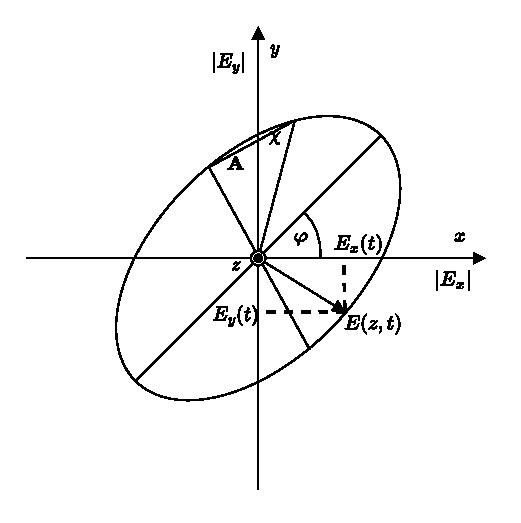
\includegraphics[width=7.3cm]{pic/chapter2/极化椭圆示意图.pdf}
    \caption{极化椭圆示意图\citing{皮亦鸣2007合成孔径雷达成像原理}}
    \label{极化椭圆示意图}
\end{figure}

由公式\eqref{轨迹方程}在$z_0$处的运动轨迹可以得到极化椭圆,如图\ref{极化椭圆示意图}所示。对于任意一个极化椭圆。可以通过椭圆幅度$A$,椭圆方向角$\chi \in [-\frac{\pi}{4}, \frac{\pi}{4}]$和椭圆孔径$\varphi \in [-\frac{\pi}{2}, \frac{\pi}{2}]$进行唯一表示:
\begin{gather}
    \bf{A}=\sqrt{\left|E_{x_0}\right|^2+\left|E_{y_0}\right|^2}                                                                \\
    \tan 2 \varphi=\frac{2\left|E_{x_0}\right|\left|E_{y_0}\right|^2}{\left|E_{x_0}\right|^2-\left|E_{y_0}\right|^2} \cos (\delta) \\
    \sin 2 \chi=\frac{2\left|E_{x_0}\right|\left|E_{y_0}\right|^2}{\left|E_{x_0}\right|^2+\left|E_{y_0}\right|^2} \sin (\delta)
\end{gather}
根据电场矢量的旋转方向,可以将极化电磁波分为左旋和右旋两种类型。当椭圆方向角$\chi > 0$时,表示左旋极化波;当椭圆方向角$\chi < 0$时,表示左旋极化波。
\subsection{琼斯矢量}
为了简化平面电磁波极化状态的描述方式,还可以通过琼斯矢量的形式表示。将公式\eqref{平面波}使用复数的形式表示为:
\begin{equation}
    \boldsymbol{E}(z, t)=\left[\begin{array}{c}
            E_{0 x} \cos \left(\omega t-k z+\delta_x\right) \\
            E_{0 y} \cos \left(\omega t-k z+\delta_y\right)
        \end{array}\right]=\operatorname{Re}\left\{\left[\begin{array}{l}
            E_{0 x} e^{j \delta_x} \\
            E_{0 y} e^{j \delta_y}
        \end{array}\right] e^{j \omega t} e^{-j k z}\right\}
\end{equation}
其中,$Re(\cdot)$表示取实部。琼斯矢量可以定义为:
\begin{equation}
    E_{\text {Jones }}=\left[\begin{array}{l}
            E_x \\
            E_y
        \end{array}\right]=\left[\begin{array}{l}
            E_{0 x} e^{j \delta_x} \\
            E_{0 y} e^{j \delta_y}
        \end{array}\right]
\end{equation}
极化椭圆描述的极化波状态与琼斯矢量表示是等价的,可以使用椭圆极化的描述参数来表示琼斯矢量:
\begin{equation}
    E_{\text {Jones }}=\mathbf{A} e^{i a}\left[\begin{array}{l}
            \cos \varphi \cos \chi-i \sin \varphi \sin \chi \\
            \sin \varphi \cos \chi+i \cos \varphi \sin \chi
        \end{array}\right]
\end{equation}
其中,$\alpha$表示绝对相位项。琼斯矢量可以通过更加简洁的矩阵形式表示,定义为:
\begin{equation}
    E_{\text {Jones }}=\mathbf{A} e^{i a}\left[\begin{array}{cc}
            \cos \varphi & -\sin \varphi \\
            \sin \varphi & \cos \varphi
        \end{array}\right]\left[\begin{array}{c}
            \cos \chi \\
            i \sin \chi
        \end{array}\right]
\end{equation}
\subsection{Stokes矢量}
与琼斯矢量使用两个复数表示电磁波的极化状态不同,Stokes矢量使用$[g_0,g_1,g_2,g_3]$四个实数从电磁波功率的角度来描述电磁波的极化状态,Stokes参数定义如下:
\begin{equation}
    \label{Stokes}
    \left\{\begin{array}{l}
        g_0=\left|E_x\right|^2+\left|E_y\right|^2         \\
        g_1=\left|E_x\right|^2-\left|E_y\right|^2         \\
        g_2=2\left|E_x\right|\left|E_y\right| \cos \delta \\
        g_3=2\left|E_x\right|\left|E_y\right| \sin \delta
    \end{array}\right.
\end{equation}
其中,$E_x$和$E_y$分别表示电场矢量在x轴和y轴上的幅度;$\delta$表示电场矢量在x轴和y轴上的相位差;$g_0$表示电磁波总功率;$g_1$表示水平或垂直极化分量的功率;$g_2$表示$\pm 45^{\operatorname{\omicron}}$线性极化分量的功率;$g_3$表示左右旋极化分类的功率之和。

可以使用极化椭圆参数表示公式\eqref{Stokes},具体如下:
\begin{equation}
    \boldsymbol{g}=\left[\begin{array}{c}
            A^2                             \\
            A^2 \cos (2 \phi) \cos (2 \tau) \\
            A^2 \sin (2 \phi) \cos (2 \tau) \\
            A^2 \sin (2 \tau)
        \end{array}\right]
\end{equation}

\section{极化散射数据表示方式}
极化SAR系统通过发射水平和垂直两种不同极化方式的电磁波,对目标进行探测,当电磁波遇到目标后,部分被目标体吸收,另外一部分通过目标辐射,形成反射回波。由于散射回波因目标的散射特性而异,因此可以通过分析回波的特性来推断目标的特征。为了能够表征目标的极化散射特性,需要引入不同的参数来描述各个极化通道散射回波在幅度相位上的差异。
\subsection{极化散射矩阵和Mueller矩阵}
极化SAR系统从发射的不同极化形式的电磁波信号,到以不同的极化方式接收经过目标反射的电磁波,目标的反射过程可以看做电磁波对应琼斯矢量的线性转换的过程。为了描述这个线性转换的过程,引入极化散射矩阵\citing{sinclair1950transmission},又称为Sinclair矩阵,简写为$\textbf{S}$,通常使用$2\times2$的复数矩阵表示,具体如下:
\begin{equation}
    \textbf{S}  =\left[ \begin{matrix}
            S_{\mathrm{HH}} & S_{\mathrm{HV}} \\
            S_{\mathrm{VH}} & S_{\mathrm{VV}} \\
        \end{matrix} \right]
\end{equation}
其中,$\mathrm{H}$和$\mathrm{V}$分别表示水平和垂直的极化方式,$S_{\text{XY}}(\text{X,Y=H,V})$表示发射$\text{X}$极化波、接收$\text{Y}$极化波的后向散射系数,在满足单站互易条件下,$S_{\mathrm{HV}}=S_{\mathrm{VH}}$。此时,极化散射矩阵可以表示为如下形式:
\begin{equation}
    \textbf{S}  =\left[ \begin{matrix}
            S_{\mathrm{HH}} & S_{\mathrm{HV}} \\
            S_{\mathrm{HV}} & S_{\mathrm{VV}} \\
        \end{matrix} \right]
\end{equation}

以上的极化散射矩阵适用于表述完全极化波对应的琼斯矢量的入射与散射之间的线性关系,但是通常情况下,入射与散射的电磁波都是部分极化电磁波,这种情况下,需要引入Mueller矩阵\citing{guissard1994mueller}来进行表示它们之间的关系。

Mueller矩阵是一个$4\times4$的矩阵,简写为$\textbf{M}$,具体表示如下:
\begin{equation}
    \label{Mueller}
    \textbf{M}=\textbf{R}\left( \textbf{S}\otimes \textbf{S}^* \right) \textbf{R}^{-1}
\end{equation}
其中,$\textbf{S}$是Sinclair矩阵,$\textbf{R}$是转换系数矩阵,具体如下:
\begin{equation}
    \label{R}
    \textbf{R}=\left[ \begin{matrix}
            1 & 0 & 0  & 1  \\
            1 & 0 & 0  & -1 \\
            0 & 1 & 1  & 0  \\
            0 & i & -i & 0  \\
        \end{matrix} \right]
\end{equation}

从公式\eqref{Mueller}和公式\eqref{R}可以看出,$\textbf{M}$实际上是经过$\textbf{S}$运算得到,因此$\textbf{M}$与$\textbf{S}$属于一一对应的关系,但是$\textbf{S}$相比于$\textbf{M}$还多具备了绝对的相位信息。

\subsection{极化相干矩阵和协方差矩阵}
在极化SAR系统成像过程中,目标的散射回波通常会受到周围环境中其他散射体产生的杂波的干扰。为了减少散射杂波的影响,实践中尝尝采用矢量化分解对极化散射矩阵$\textbf{S}$进行处理,导出描述二阶统计特性的极化相干矩阵和极化协方差矩阵。

通常利用正交的矩阵基来对极化散射矩阵进行矢量化分解,矢量化过程表示如下:
\begin{equation}
    \textbf{S}=\left[ \begin{matrix}
            S_{\mathrm{HH}} & S_{\mathrm{HV}} \\
            S_{\mathrm{HV}} & S_{\mathrm{VV}} \\
        \end{matrix} \right] \Rightarrow \textbf{K}_4=\text{V(\textbf{S})}=\frac{1}{2}\mathrm{Trace(}\textbf{S}\Psi )=\left[ k_0,k_1,k_2,k_3 \right] ^\mathrm{T}
\end{equation}
其中,$\text{V}(\cdot)$表示矢量化操作,$\text{Trace}(\cdot)$表示矩阵求迹,$\Psi$表示$2\times2$的复单位矩阵,$\mathrm{T}$表示矩阵转置。最常用的有两组标准基,分别是Lexicograhic基$\Psi_L$和Pauli基$\Psi_p$,具体如下:
\begin{gather}
    \Psi_L=\left\{\left[\begin{array}{ll}
            2 & 0 \\
            0 & 0
        \end{array}\right],\left[\begin{array}{ll}
            0 & 2 \\
            0 & 0
        \end{array}\right],\left[\begin{array}{ll}
            0 & 0 \\
            2 & 0
        \end{array}\right],\left[\begin{array}{ll}
            0 & 0 \\
            0 & 2
        \end{array}\right]\right\}                                    \\
    \Psi_P=\left\{\sqrt{2}\left[\begin{array}{ll}
            1 & 0 \\
            0 & 1
        \end{array}\right], \sqrt{2}\left[\begin{array}{cc}
            1 & 0  \\
            0 & -1
        \end{array}\right], \sqrt{2}\left[\begin{array}{ll}
            0 & 1 \\
            1 & 0
        \end{array}\right], \sqrt{2}\left[\begin{array}{cc}
            0 & -i \\
            i & 0
        \end{array}\right]\right\}
\end{gather}

基于以上两组基,分别得到目标散射矢量:
\begin{gather}
    \label{4L}
    \textbf{k}_{\textbf{4L}}=\left[S_{\mathrm{HH}}, S_{\mathrm{HV}}, S_{\mathrm{VH}}, S_{\mathrm{VV}}\right] \\
    \label{4P}
    \textbf{k}_{\textbf{4P}}=\frac{1}{\sqrt{2}}\left[S_{\mathrm{HH}}+S_{\mathrm{VV}}, S_{\mathrm{HH}}-S_{\mathrm{VV}}, S_{\mathrm{HV}}+S_{\mathrm{VH}}, i\left(S_{\mathrm{HV}}+S_{\mathrm{VH}}\right)\right]
\end{gather}

由单站互易定理可知$S_{\mathrm{HV}}=S_{\mathrm{VH}}$,可以将公式\eqref{4L}和\eqref{4P}简写为:
\begin{equation}
    \begin{gathered}
        \textbf{k}_{\textbf{3L}}=\left[S_{\mathrm{HH}}, \sqrt{2}S_{\mathrm{HV}}, S_{\mathrm{VV}}\right] \\
        \textbf{k}_{\textbf{3P}}=\frac{1}{\sqrt{2}}\left[S_{\mathrm{HH}}+S_{\mathrm{VV}}, S_{\mathrm{HH}}-S_{\mathrm{VV}}, 2S_{\mathrm{HV}}\right]
    \end{gathered}
\end{equation}

通过计算散射矢量$\textbf{k}_{\textbf{3L}}$与其复共轭转置矢量$\textbf{k}_{\textbf{3L}}^{\text{H}}$的内积可以得到极化协方差矩阵$\textbf{C}$,具体表示如下:
\begin{equation}
    \textbf{C}=\left. \langle \textbf{k}_{\textbf{3L}}\cdot \textbf{k}_{\textbf{3L}}^{^*\boldsymbol{H}} \right. \rangle =\left[ \begin{matrix}
            \left. \langle \left. S_{\mathrm{HH}} \right|^2 \right. \rangle           & \left. \langle \sqrt{2}S_{\mathrm{HH}}S_{\mathrm{HV}}^{*} \right. \rangle  & \left. \langle S_{\mathrm{HH}}S_{\mathrm{VV}}^{*} \right. \rangle         \\
            \left. \langle \sqrt{2}S_{\mathrm{HV}}S_{\mathrm{HH}}^{*} \right. \rangle & \left. \langle 2\left| S_{\mathrm{HV}} \right|^2 \right. \rangle           & \left. \langle \sqrt{2}S_{\mathrm{HV}}S_{\mathrm{VV}}^{*} \right. \rangle \\
            \left. \langle S_{\mathrm{VV}},S_{\mathrm{HH}}^{*} \right. \rangle        & \left. \langle \sqrt{2}S_{\mathrm{VV}},S_{\mathrm{HV}}^{*} \right. \rangle & \left. \langle \left| S_{\mathrm{VV}} \right|^2 \right. \rangle           \\
        \end{matrix} \right]
\end{equation}

同理,通过计算散射矢量$\textbf{k}_{\textbf{3P}}$与其复共轭转置矢量$\textbf{k}_{\textbf{3P}}^\text{H}$的内积可以得到极化相干矩阵$\textbf{T}$,具体表示如下:
\begin{equation}
    \label{eq:T}
    \begin{aligned}
        \textbf{T} & =\left. \langle \textbf{3P}\cdot\textbf{3P}^{^*\text{H}} \right. \rangle                                                                                                                                                                                                                                                                                                                                                                                                                                                                                                                              \\
                   & =\frac{1}{2}\left[ \begin{matrix}
                                                \langle \left| S_{\mathrm{HH}}+S_{\mathrm{VV}} \right|^2\rangle                                                                 & \left. \langle \left( S_{\mathrm{HH}}+S_{\mathrm{VV}} \right) \left( S_{\mathrm{HH}}-S_{\mathrm{VV}} \right) ^* \right. \rangle & \left. \langle 2\left( S_{\mathrm{HH}}+S_{\mathrm{VV}} \right) S_{\mathrm{HV}}^{*} \right. \rangle \\
                                                \left. \langle \left( S_{\mathrm{HH}}-S_{\mathrm{VV}} \right) \left( S_{\mathrm{HH}}+S_{\mathrm{VV}} \right) ^* \right. \rangle & \left. \langle \left| S_{\mathrm{HH}}-S_{\mathrm{VV}} \right|^2 \right. \rangle                                                 & \left. \langle 2\left( S_{\mathrm{HH}}-S_{\mathrm{VV}} \right) S_{\mathrm{HV}}^{*} \right. \rangle \\
                                                \left. \langle 2S_{\mathrm{HV}}\left( S_{\mathrm{HH}}+S_{\mathrm{VV}} \right) ^* \right. \rangle                                & \left. \langle 2S_{\mathrm{HV}}\left( S_{\mathrm{HH}}-S_{\mathrm{VV}} \right) ^* \right. \rangle                                & \left. \langle 4\left| S_{\mathrm{HV}} \right|^2 \right. \rangle                                   \\
                                            \end{matrix} \right]
    \end{aligned}
\end{equation}
其中,$\langle \cdot \rangle$表示取总体平均,$(\cdot)^*$和$(\cdot)^\text{T}$分别表示复共轭和矩阵转置。

极化协方差矩阵$\textbf{C}$与极化相干矩阵$\textbf{T}$都具备半正定的Hermitain(即埃尔米特)特性,两者之间可以相互转换,计算过程如下式所示:
\begin{gather}
    \textbf{C}=\textbf{U}^\text{H} \textbf{T} \textbf{U}=\textbf{U}^{-1} \textbf{T} \textbf{U} \\
    \textbf{T}=\textbf{U} \textbf{C} \textbf{U}^\text{H}=\textbf{U} \textbf{C} \textbf{U}^{-1}
\end{gather}
其中,$\textbf{U}$表示单位转换矩阵,具体可以表示为:
\begin{equation}
    \textbf{U}=\frac{1}{\sqrt{2}}\left[ \begin{matrix}
            1 & 0        & 1  \\
            1 & 0        & -1 \\
            0 & \sqrt{2} & 0  \\
        \end{matrix} \right]
\end{equation}

\section{极化目标分解理论基础}
极化散射矩阵全面的描述了目标的散射特征,可以从中获取到目标表面粗糙度、对称性以及取向性等信息,为深层次地探索目标特性提供了数据支撑。但是,仅仅基于测量到的散射数据并无法直接获取丰富的信息,还需要进一步对测量的散射矩阵进行数据处理,进而从其中提取出能表征目标特征的极化描述。为了更清晰的描述不同目标的极化特性,可以将散射矩阵通过不同的散射模型作为基分解为几个矩阵的线性组合,由于这些基础散射模型具有不同的物理意义,分解矩阵可以表示目标的不同散射特性,为分类识别任务提供更加充分、全面的极化信息。根据处理数据的不同,极化目标分解方法可以分类相干分解和非相干分解两种类型。极化目标分解根据分解的数据分为相干分解和非相干分解两种类别:相干分解的分对象是极化散射矩阵,要求目标具有稳定的散射性质和相干的散射波;非相干分解的分解对象是极化相干矩阵或极化协方差矩阵,要求目标具有非相干散射波,散射的特征随时间变化,探测目标可以是分布式目标。
\subsection{极化相干分解}
极化相干分解的基本思想是通过不同的基础散射模型,将测量得到的散射矩阵分解成多个散射机制之和,如下式所示:
\begin{equation}
    \textbf{S}=\sum_{k=1}^N{a_k\textbf{S}_k}
\end{equation}
其中,$\textbf{S}$表示极化散射矩阵,$\textbf{S}_k$表示分解得到的经典目标的散射矩阵,$a_k$表示对应的权值。

经典的极化相干分解方法有Pauli分解\citing{cloude1996review}、Krogager分解\citing{krogager1990new}、Cameron分解\citing{cameron1990feature}、球坐标分解\citing{lee2017polarimetric}等。下面将介绍Pauli分解和Krogager分解的基本原理。
\subsubsection{Pauli分解}
Pauli分解方法是使用Pauli基对极化散射矩阵进行分解,分解过程如下式所示:
\begin{equation}
    \textbf{S}=\left[ \begin{matrix}
            S_{\mathrm{HH}} & S_{\mathrm{HV}} \\
            S_{\mathrm{VH}} & S_{\mathrm{VV}} \\
        \end{matrix} \right] =a\textbf{S}_a+b\textbf{S}_b+c\textbf{S}_c+d\textbf{S}_d
\end{equation}
其中,$a,b,c,d$均是权重系数,$\textbf{S}_a,\textbf{S}_b,\textbf{S}_c,\textbf{S}_d$表示Pauli基,具体如下式所示:
\begin{equation}
    \textbf{S}_a=\left[ \begin{matrix}
            1 & 0 \\
            0 & 1 \\
        \end{matrix} \right] ,\textbf{S}_b=\left[ \begin{matrix}
            1 & 0  \\
            0 & -1 \\
        \end{matrix} \right] ,\textbf{S}_c=\left[ \begin{matrix}
            0 & 1 \\
            1 & 0 \\
        \end{matrix} \right] ,\textbf{S}_d=\left[ \begin{matrix}
            0 & -i \\
            i & 0  \\
        \end{matrix} \right]
\end{equation}

权重系数使用向量的形式,可以表示为:
\begin{equation}
    \textbf{K}=\left[ \begin{matrix}
            a & b & c & d \\
        \end{matrix} \right] =\frac{1}{\sqrt{2}}\left[ \begin{matrix}
            S_{\mathrm{HH}}+S_{\mathrm{VV}} & S_{\mathrm{HH}}-S_{\mathrm{VV}} & S_{\mathrm{HV}}+S_{\mathrm{VH}} & i\left( S_{\mathrm{VH}}-S_{\mathrm{HV}} \right) \\
        \end{matrix} \right] ^T
\end{equation}

满足单站互易条件时,可以简化为:
\begin{equation}
    \textbf{S}\textbf{S}=\left[ \begin{matrix}
            a & b & c \\
        \end{matrix} \right] =\frac{1}{\sqrt{2}}\left[ \begin{matrix}
            S_{\mathrm{HH}}+S_{\mathrm{VV}} & S_{\mathrm{HH}}-S_{\mathrm{VV}} & 2S_{\mathrm{HV}} \\
        \end{matrix} \right] ^T
\end{equation}

对于Pauli分解的每个分量的物理解释如表\ref{Pauli table}所示。
\begin{table}[ht!]
    \caption{Pauli分解}
    % \linespread{1.5} % 调整整个表格的行高
    % \setlength{\arraycolsep}{10pt} % 调整列之间的空白
    \begin{tabular}{ccc}
        \toprule[1.5bp]
        Pauli基                 & 散射类型                & 物理描述                             \\
        \midrule[0.75bp]
        $\left[ \begin{matrix}
                            1 & 0 \\
                            0 & 1 \\
                        \end{matrix} \right] $ & 奇次散射                & 球体、平坦平面或三面角反射器           \\
        $\left[ \begin{matrix}
                            1 & 0  \\
                            0 & -1 \\
                        \end{matrix} \right] $ & 偶次散射                & 二面角反射器                   \\
        $\left[ \begin{matrix}
                            0 & 1 \\
                            1 & 0 \\
                        \end{matrix} \right] $ & $\frac{\pi}{4}$偶次散射 & 与水平$\frac{\pi}{4}$倾角的二面角 \\
        \bottomrule[1.5bp]
    \end{tabular}
    \label{Pauli table}
\end{table}
% \begin{figure}[h]
% 	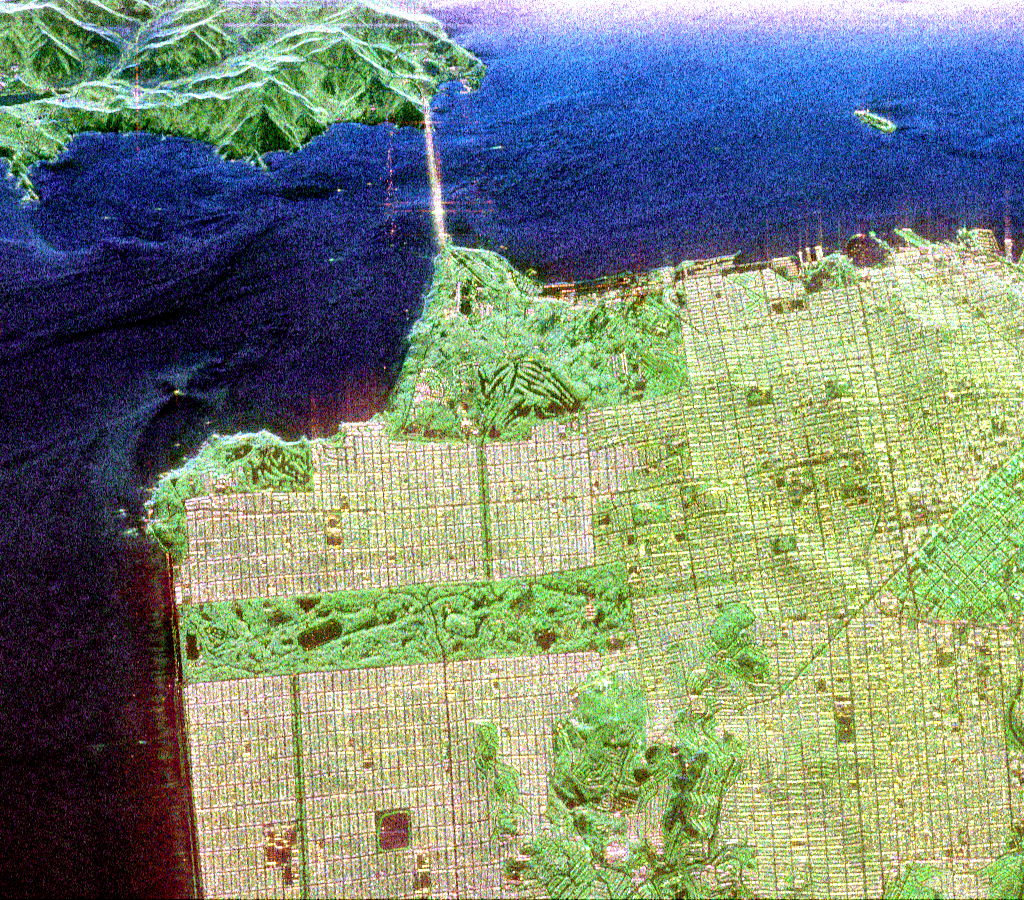
\includegraphics[width=7.3cm]{pic/chapter2/SF-Puali.jpg}
% 	\caption{Pauli分解伪彩图(R:$ \left | a \right |^2$,G:$ \left | b \right |^2$,B:$ \left | c \right |^2$)}
% 	\label{Pauli示意图}
% \end{figure}

\subsubsection{Krogager分解}
Krogager分解是将极化散射矩阵$\textbf{S}$分解为球散射、二面角散射以及螺旋体散射三个散射分量的加权和,具体如下:
\begin{equation}
    \begin{aligned}
        \textbf{S} & =e^{j \phi}\left\{e^{j \phi_S} k_S \textbf{S}_{sphere}+k_D \textbf{S}_{diplane(\theta)}+k_H \textbf{S}_{helix(\theta)}\right\}                 \\
                   & =e^{j \phi}\left\{e^{j \phi_S} k_S\left[\begin{array}{ll}
                                                                     1 & 0 \\
                                                                     0 & 1
                                                                 \end{array}\right]+k_D\left[\begin{array}{cc}
                                                                                                 \cos 2 \theta & \sin 2 \theta  \\
                                                                                                 \sin 2 \theta & -\cos 2 \theta
                                                                                             \end{array}\right]+k_H e^{ \pm j 2 \theta}\left[\begin{array}{cc}
                                                                                                                                                 1     & \pm j \\
                                                                                                                                                 \pm j & -1
                                                                                                                                             \end{array}\right]\right\}
    \end{aligned}
\end{equation}
其中,$k_s$、$k_D$、$k_H$分别表示各个分量的权值,也被称作能量;$\theta$表示取向角;$\phi$表示散射矩阵的绝对相位。

当电磁波以左旋圆极化方式发射,右旋圆极化接收时,Krogager分解可以表示为:
\begin{equation}
    \begin{aligned}
        \textbf{S}_{(R,L)} & =\left[ \begin{matrix}
                                             \textbf{S}_{RR} & \textbf{S}_{RL} \\
                                             \textbf{S}_{LR} & \textbf{S}_{LL} \\
                                         \end{matrix} \right]
        \\
                           & =e^{j\phi}\left\{ e^{j\phi _S}k_S\left[ \begin{matrix}
                                                                             0 & j \\
                                                                             j & 0 \\
                                                                         \end{matrix} \right] +k_D\left[ \begin{matrix}
                                                                                                             e^{j2\theta} & j              \\
                                                                                                             j            & -e^{-j2\theta} \\
                                                                                                         \end{matrix} \right] +k_H\left[ \begin{matrix}
                                                                                                                                             e^{j2\theta} & 0 \\
                                                                                                                                             0            & 0 \\
                                                                                                                                         \end{matrix} \right] \right\}
    \end{aligned}
\end{equation}
其中,Krogager的参数可以表示为:
\begin{equation}
    \label{Krogager参数}
    \begin{matrix}
        k_S=\left| \textbf{S}_{RL} \right|,                           & \phi =\frac{1}{2}\left( \phi _{RR}+\phi _{LL}-\pi \right)          \\
        \theta =\frac{1}{4}\left( \phi _{RR}-\phi _{LL}+\pi \right) , & \phi _S=\phi _{RL}-\frac{1}{2}\left( \phi _{RR}+\phi _{LL} \right) \\
    \end{matrix}
\end{equation}

从公式\eqref{Krogager参数}可以看出,目标的左右旋散射特性可以由$\textbf{S}_{RR}$和$\textbf{S}_{LL}$确定。当目标为左螺旋体时:
\begin{equation}
    \left| \textbf{S}_{RR} \right|\geqslant \left| \textbf{S}_{LL} \right|\Rightarrow \left\{ \begin{array}{c}
        k_{D}^{+}=\left| \textbf{S}_{LL} \right|                                \\
        k_{H}^{+}=\left| \textbf{S}_{RR} \right|-\left| \textbf{S}_{LL} \right| \\
    \end{array} \right.
\end{equation}

类似地,当目标为右螺旋体时:
\begin{equation}
    \left| \textbf{S}_{RR} \right|\leqslant \left| \textbf{S}_{LL} \right|\Rightarrow \left\{ \begin{array}{c}
        k_D=\left| \textbf{S}_{RR} \right|                                \\
        k_H=\left| \textbf{S}_{LL} \right|-\left| \textbf{S}_{RR} \right| \\
    \end{array} \right.
\end{equation}

Krogager分解每个分量的物理解释如表\ref{Krogager table}所示。
\begin{table}[h]
    \caption{Krogager分解}
    \begin{tabular}{ccc}
        \toprule[1.5bp]
        Krogager基                   & 散射类型  & 物理描述                   \\
        \midrule[0.75bp]
        $\left[ \begin{matrix}
                            1 & 0 \\
                            0 & 1 \\
                        \end{matrix} \right] $      & 球面散射  & 球体、平坦平面或三面角反射器 \\
        $\left[ \begin{matrix}
                            cos2\theta & sin2\theta  \\
                            sin2\theta & -cos2\theta \\
                        \end{matrix} \right] $ & 二面角散射 & 二面角反射器              \\
        $\left[ \begin{matrix}
                            1     & \pm j \\
                            \pm j & -1    \\
                        \end{matrix} \right] $      & 螺旋体散射 & 不对称结构          \\
        \bottomrule[1.5bp]
    \end{tabular}
    \label{Krogager table}
\end{table}

\subsection{极化非相干分解}
对于“非确定性”的非相干目标,具有动态的散射特性,因此需要使用统计的方法来对其目标散射特性进行研究,通常是使用二阶统计量的方法展开。非相干分解主要是将极化协方差矩阵$\textbf{C}$或者极化相干矩阵$\textbf{T}$进行分解,使用多个典型的散射模型之和的形式表示。
\begin{gather}
    \textbf{C}=\sum_{k=1}^N{p_k\textbf{C}_k}
    \\
    \textbf{T}=\sum_{k=1}^N{q_k\textbf{T}_k}
\end{gather}
其中,$p_k$和$q_k$均表示每个散射模型分量的权重系数。

经典的非相干分解方法包括Cloude分解\citing{cloude1997entropy}、Freeman分解\citing{freeman1998three}、Huynen分解\citing{huynen1988extraction}、Yamaguchi分解\citing{yamaguchi2005four}、Holm分解\citing{holm1988radar}和van Zyl分解\citing{van1993application}等。下面将介绍Cloude分解和Freeman分解的原理。
\subsubsection{Cloude分解}
Cloude分解是一种矩阵特征空间分解方法,是对极化相干矩阵$\textbf{T}$进行特征分解,得到三组特征值与对应的特征向量。具体如下式所示:
\begin{equation}
    \textbf{T}=\textbf{U} \Lambda \textbf{U}^{\text{H}}=\textbf{U}\left[\begin{array}{ccc}
            \lambda_1 & 0         & 0         \\
            0         & \lambda_2 & 0         \\
            0         & 0         & \lambda_3
        \end{array}\right] \textbf{U}^{\text{H}}
\end{equation}
其中,$\Lambda$表示矩阵$\textbf{T}$的三个特征值组成的对角矩阵,并且满足$\lambda_1 \geqslant \lambda_2 \geqslant \lambda_3 \geqslant 0$,$\textbf{U}$表示三个特征值对应的特征向量构成的矩阵,$\text{H}$表示取复共轭转置。

由以上的特征值与特征向量,Cloude分解定义了平均散射角$\bar{a}$、极化熵$H$以及极化反熵$A$这三个用于描述目标统计的散射机制的量,具体如下表示:
\begin{gather}
    \bar{\alpha}=\sum_{i=1}^3{P_i\alpha _i}
    \\
    H=\sum_{i=1}^3{P_i\log _3P_i}
    \\
    A=\frac{\lambda _2-\lambda _3}{\lambda _2+\lambda _3}
\end{gather}
其中,$\alpha_i$表示从特征值$\lambda_i$中得到的散射角,$P_i=\frac{\lambda _i}{\sum_j{\lambda _j}}$。

从Cloude分解的三个散射分类计算式可以看出,平均散射角$\bar{\alpha}$描述了散射角从$0^{\operatorname{\omicron}}$到$90^{\operatorname{\omicron}}$变化过程中,散射特性从单次散射到二面角散射的连续变化的过程;极化熵$H$描述了目标散射特性的随机性,当$H=1$时,目标是一个随机噪声,当$H=0$时,目标的散射特性唯一,相当于一个相干目标;极化反熵$A$是对极化熵的补充量,通常用来作为极化熵难以区分目标的指标量。

Cloude分解每个分量的物理解释如表\ref{Cloude table}所示。
\begin{table}[h]
    \caption{Cloude分解}
    \begin{tabular}{ccc}
        \toprule[1.5bp]
        Cloude参数         & 参数表达                                                    & 物理描述                  \\
        \midrule[0.75bp]
        Entropy          & $H=\sum_{i=1}^3{P_i\log _3P_i}$                         & 散射目标由各向性散射至完全随机散射的随机性 \\
        Mean Alpha Angle & $\bar{\alpha}=\sum_{i=1}^3{P_i\alpha _i}$               & 由表面散射至二面角散射的平均随机性     \\
        Anisotropy       & $A=\frac{\lambda _2-\lambda _3}{\lambda _2+\lambda _3}$ & 主散射体之外的两个较弱散射分量的强弱关系  \\
        \bottomrule[1.5bp]
    \end{tabular}
    \label{Cloude table}
\end{table}

\subsubsection{Freeman分解}
Freeman和Durden基于van Zyl的目标分解工作,进一步提出了一种非相干的三分量分解方法,将极化协方差矩阵$\textbf{C}$使用单次散射、偶次散射和体散射三种散射机制的加权和表示。具体表示如下:
\begin{equation}
    \textbf{C}=f_s\textbf{C}_s+f_d\textbf{C}_d+f_v\textbf{C}_v
\end{equation}
其中,
\begin{equation}
    \begin{matrix}
        \textbf{C}_s=\left[ \begin{matrix}
                                    \left| \beta \right|^2 & 0 & \beta \\
                                    0                      & 0 & 0     \\
                                    \beta ^*               & 0 & 1     \\
                                \end{matrix} \right] , & \textbf{C}_d=\left[ \begin{matrix}
                                                                                 \left| \alpha \right|^2 & 0 & \alpha \\
                                                                                 0                       & 0 & 0      \\
                                                                                 \alpha ^*               & 0 & 1      \\
                                                                             \end{matrix} \right] , & \textbf{C}_v=\left[ \begin{matrix}
                                                                                                                              1   & 0   & 1/3 \\
                                                                                                                              0   & 2/3 & 0   \\
                                                                                                                              1/3 & 0   & 1   \\
                                                                                                                          \end{matrix} \right] \\
    \end{matrix}
\end{equation}
其中$\beta$ 表示单次散射参数,$\alpha$ 表示偶次散射参数;$\textbf{C}_s$、$\textbf{C}_d$、$\textbf{C}_v$分别表示单次散射模型、偶次散射模型和体散射模型的协方差矩阵分量;$f_s$、$f_d$,$f_v$表示三种散射模型对应的分解系数。

Freeman分解每个分量的物理解释如表\ref{Freeman table}所示。
\begin{table}[!ht]
    \caption{Freeman分解}
    \begin{tabular}{ccc}
        \toprule[1.5bp]
        Freeman基                                   & 散射类型 & 典型散射体 \\
        \midrule[0.75bp]
        $\left[ \begin{matrix}
                            \left| \beta \right|^2 & 0 & \beta \\
                            0                      & 0 & 0     \\
                            \beta ^*               & 0 & 1     \\
                        \end{matrix} \right]$      & 单次散射 & 一阶Bragg表面散射体  \\
        $\left[ \begin{matrix}
                            \left| \alpha \right|^2 & 0 & \alpha \\
                            0                       & 0 & 0      \\
                            \alpha ^*               & 0 & 1      \\
                        \end{matrix} \right]$    & 偶次散射 & 二面角散射器          \\
        $\left[ \begin{matrix}
                            1           & 0           & \frac{1}{3} \\
                            0           & \frac{2}{3} & 0           \\
                            \frac{1}{3} & 0           & 1           \\
                        \end{matrix} \right]$ & 体散射  & 植被冠状层偶极子           \\
        \bottomrule[1.5bp]
    \end{tabular}
    \label{Freeman table}
\end{table}

\section{本章小结}
本章详细介绍了极化电磁波和极化散射数据的理论基础。首先,阐述了电磁波极化的三种描述方法:极化椭圆、用于描述完全极化波的琼斯矢量,以及用于描述部分极化波的Stokes矢量。其次,介绍了用于描述目标散射特征的方法,包括极化散射矩阵以及二阶统计矩阵。然后,详尽阐述了多种极化目标分解方法的基本原理,并总结归纳了各种目标分解参数的物理含义。本章旨在为后续章节中极化SAR图像目标分类方法研究提供理论支撑。